\rhead{\itshape Résultat et mise en oeuvre}
\chapter{Résultat et mise en oeuvre}

\section{Introduction}
Dans le processus du développement, l’implémentation d’un logiciel vient après un enchainement de plusieurs étapes et son but principal est de réaliser un produit capable de résoudre les problèmes posés en utilisant des outils et des algorithmes.


Dans le but de réaliser et valider les idées proposées dans le chapitre 4, le présent chapitre montre les outils et les configurations utilisées afin de développer ce système.


Dans ce chapitre nous allons présenter les outils et les plateformes utilisés pour développer notre approche. Ensuite, nous présentons quelques interfaces qui montrent les résultats obtenus. Puis, nous présentons une discussion sur les résultats pour chaque évaluation.
\section{Outils et plateformes utilisés}
Dans cette section, nous allons présenter les plateformes utilisées afin de réaliser notre système. Les implémetations ont été réalisées en utilisant un ordinateur de processeur Core I3 avec une RAM de 8 Go sous Windows 7, mais on peut implémenter ce système sur n’importe quelle machine grâce à la machine virtuelle du Java.

Pour développer les agents, nous avons utilisés la plateforme JADE, grâce aux avantages du cette dernière qui nous offre un langage de communication entre les agents en utilisant le FIPA-ACL. Afin de simuler les idées proposées, nous avons créé une plateforme pour simuler les ressources virtuelles d’un smart-home ainsi que les tâches réalisées dans notre système.
\section{Plateforme JADE}
Afin d’assurer le bon fonctionnement de notre systéme et à cause de la nature de notre architecture qui est basée sur les agents, nous avons utilisé la plateforme de développement des systèmes multi -agent JADE, qui comporte un ensemble d’outils et d’API qui permettent la construction et la mise en service des agents sur un contexte bien spécifique.
\subsection{Présentation générale}
JADE est une plateforme implémentée avec le langage JAVA. Ce Framework est destiné aux développeurs qui s’intéressent à créer des systèmes multi-agents, et qui assure un langage de communication prédéfini et représenté dans les standards FIPA-ACL. Parmi les avantages offerts par la plateforme JADE ; l’interopérabilité sans limite pour les applications quelles prennent en charge, et l’indépendance de cette plateforme du système d’exploitation ou du matériel sur laquelle elle est implémentée \cite{36}. JADE est composée de trois principaux modules qui dépendent directement des normes FIPA :
\begin{itemize}
    \item \textbf{DF :} pour Directory Facilitator en anglais, qui sert à la fourniture d’un service de «page jaune» à toute la plateforme JADE.
    \item \textbf{ACC :} pour Agent Communication Channel en anglais, qui représente l’outil de gestion de communication entre agents, pour la plateforme JADE.
    \item \textbf{AMS :} pour Agent Management System en anglais, qui représente l’outil de gestion (authentification, supervision, accès ... etc.) des agents de la plateforme JADE.

\end{itemize}
\subsection{Architecture du logiciel}
JADE est une plateforme basée sur les standards FIPA. En outre, le modèle de base de l’architecture de la plateforme JADE proposée par FIPA est intitulé AMRM (Agent Management Reference Model en anglais). Chaque module, qui compose l’architecture de cette plateforme, est présenté sous forme de service, ce qui permet aux agents de bénéficier d’une plateforme orientée service, afin de faciliter la communication et la collaboration entre eux \cite{37}.


Afin d’assurer un fonctionnement efficace des agents sur la plateforme JADE, cette dernière utilise :
\begin{itemize}
    \item \textbf{AID :} pour Agent Identifier en anglais, afin de distinguer et d’identifier chaque agent.
    \item \textbf{DF :} joue le rôle d’un annuaire qui enregistre les compétences de chaque agent. Les pages jaunes fournis par ce service, sont destinées à mettre en relation les différents agents fonctionnels sur la plateforme JADE, et cela pour qu’un agent puisse consulter et interroger ce service, afin d’obtenir des informations sur les compétences des autres agents et par conséquent, d’assurer une bonne collaboration entre eux.
    \item \textbf{AMS :} joue le rôle d’un annuaire pour l’enregistrement des adresses de transport des différents agents de la plateforme. Le but est de fournir un service de «pages blanches» afin de mettre en correspondance les agents avec l’AID, pour faciliter leur contrôle et supervision.
\end{itemize}
\section{Simulateur smart house}
Le simulateur  est une API de simulation de maison intelligente basée sur le langage Java et une interface graphique très riche créée par le langage JavaFX, cette interface fournit au programmeur et au chercheur un environnement pour simuler une maison intelligente. Il lui donne également le contrôle des appareils électroménagers virtuels.

Dans notre environnement, nous avons six IoT VD, chaque appareil a deux méthodes principales:

\begin{enumerate}
   
\item \textbf{Méthode d'affectation des états:} il s'agit d'une méthode pour modifier l'état du périphérique \textit{(ON, OFF, SUSPENDU)} pendant le fonctionnement de l'environnement sans relancer l'exécution de l'API;
Le statut à passer comme paramètre dans la méthode Set (états), pour appeler la méthode set dans une autre classe, procédez comme suit:


\begin{center}
\textit{Name of Main Class (.) LinFiSim instance (.) Set\_Method(status)}
\end{center}
\begin{lstlisting}
MainClass.L.Set_LAMP_1_Status(Status.start);//Example
\end{lstlisting}
Le climatiseur virtuel a deux autres méthodes définies: la température définie et l'humidité définie qui définissent les valeurs pour stabiliser la température et l'humidité de l'atmosphère et de l'environnement. La température et l'humidité à passer en paramètre dans la méthode Set (\textit{int}).


L'API a une méthode Status\_show (\textit{booléenne}) qui affiche un tableau dans l'interface de simulateur pour expliquer l'état de chaque périphérique si la valeur du paramètre est vraie, le tableau est affiché sinon le tableau ne s'affiche pas.


\item \textbf{La méthode de récupération la valeur de l'état:} il s'agit d'une méthode pour obtenir l'état du périphérique (\textit{ON, OFF, SUSPENDU}) pendant le fonctionnement de l'environnement sans relancer l'exécution de l'API; la méthode get retourne l'état du périphérique, le type de valeur retournée est status, pour appeler la méthode get dans une autre classe, défine comme suit:


\textit{Status variable=Name of Main Class (.) LinFiSim instance (.) Get\_Method()}
\begin{lstlisting}
 Status s=MainClass.L.Get_LAMP_1_Status();//Example
\end{lstlisting}
\end{enumerate}
Le climatiseur virtuel  a deux autres méthodes Get: Obtenir la température et l'humidité qui obtient les valeurs de la température et de l'humidité de l'atmosphère et de l'environnement. Le type de valeur de retour est un entier.

Ce tableau définit les méthodes de chaque appareil:
\begin{table}[H]
\caption{Méthodes d'IoT VDs}
\begin{tabular}{|l|l|l|}
\hline
\multicolumn{1}{|c|}{\textbf{IoT VD}} & \multicolumn{1}{c|}{\textbf{Set Method}}                                                                                                                                  & \multicolumn{1}{c|}{\textbf{Get Method}}                                                                                                                  \\ \hline
Lamp 1                                & Set\_LAMP\_1\_Status(status)                                                                                                                                              & Get\_LAMP\_1\_Status()                                                                                                                                    \\ \hline
Lamp 2                                & Set\_LAMP\_2\_Status(status)                                                                                                                                              & Get\_LAMP\_2\_Status()                                                                                                                                    \\ \hline
Refrigerator                          & Set\_ Refrigerator\_Status(status)                                                                                                                                        & Get\_ Refrigerator \_Status()                                                                                                                             \\ \hline
Stove                                 & \begin{tabular}[c]{@{}l@{}}Set\_ Stove\_Status(status)\end{tabular}                                                                                                  & Get\_ Stove \_Status()                                                                                                                                    \\ \hline
Television                            & Set\_TV\_Status(status)                                                                                                                                                   & Get\_TV\_Status()                                                                                                                                         \\ \hline
Air conditioner                       & \begin{tabular}[c]{@{}l@{}}Set\_ AirConditioner\\   \_Status(status)\\   Set\_ AirConditioner \_ Temperature (int)\\   Set\_ AirConditioner \_ humidity(int)\end{tabular} & \begin{tabular}[c]{@{}l@{}}Get\_ AirConditioner \_Status()\\   Get\_ AirConditioner \_Temperature ()\\   Get\_ AirConditioner \_ humidity ()\end{tabular} \\ \hline
\end{tabular}
\end{table}

Dans notre environnement, nous avons également quatre IoT VS, chaque capteur possède deux méthodes principales: 

\begin{table}[H]
\centering
\caption{Méthodes de l'IoT VS}
\begin{tabular}{|l|l|l|}
\hline
\multicolumn{1}{|c|}{\textbf{IoT VS}} & \multicolumn{1}{c|}{\textbf{Set Method}} & \multicolumn{1}{c|}{\textbf{Get Method}} \\ \hline
Temperature Sensor 1                  & Set\_S1\_Temperature(int)                & Get\_S1\_Temperature()                   \\ \hline
Temperature Sensor 2                  & Set\_S2\_Temperature(int)                & Get\_S2\_Temperature()                   \\ \hline
Gas Sensor                            & Set\_Gas(booleen)                        & Get\_Gas()                               \\ \hline
Presence Sensor                       & Set\_Presence(booleen)                   & Get\_Presence()                          \\ \hline
\end{tabular}
\end{table}


\subsection{Présentation des interfaces de simulateur}
Dans cette section, nous expliquons et clarifions certaines méthodes d'appel de l'interface de programmation d'application.
\subsubsection{Lancement de l'interface graphique du simulateur}
Cette classe (MainLinfiSim) expliquer comment lancer l'interface graphique du simulateur
( Figure \ref{fc20} ), nous instancions un objet (L) du simulateur de classe (voir ligne 5) pour l'interface graphique du simulateur de spectacle, nous avons déclaré une méthode main () et nous faisons appel à la méthode publique Start\_LinfiSim(); (voir ligne 11) pour exécuter le code.
\begin{lstlisting}
1.	import java.io.IOException;
2.	import linfisim.LinFiSim;
3.	
4.	public class MainLinfiSim {
5.	public static LinFiSim L=new LinFiSim();//declaration of LinFiSim object in the main class
6.	    /**
7.	     * @param args the command line arguments
8.	     * @throws java.io.IOException
9.	     */
10.	    public static void main(String[] args) throws IOException {
11.	            L.Start_LinfiSim();//Starting the simulation window LinFiSim GUI
12.	    }
13.	    
14.	}
\end{lstlisting}


\begin{figure}[H]
    \centering
    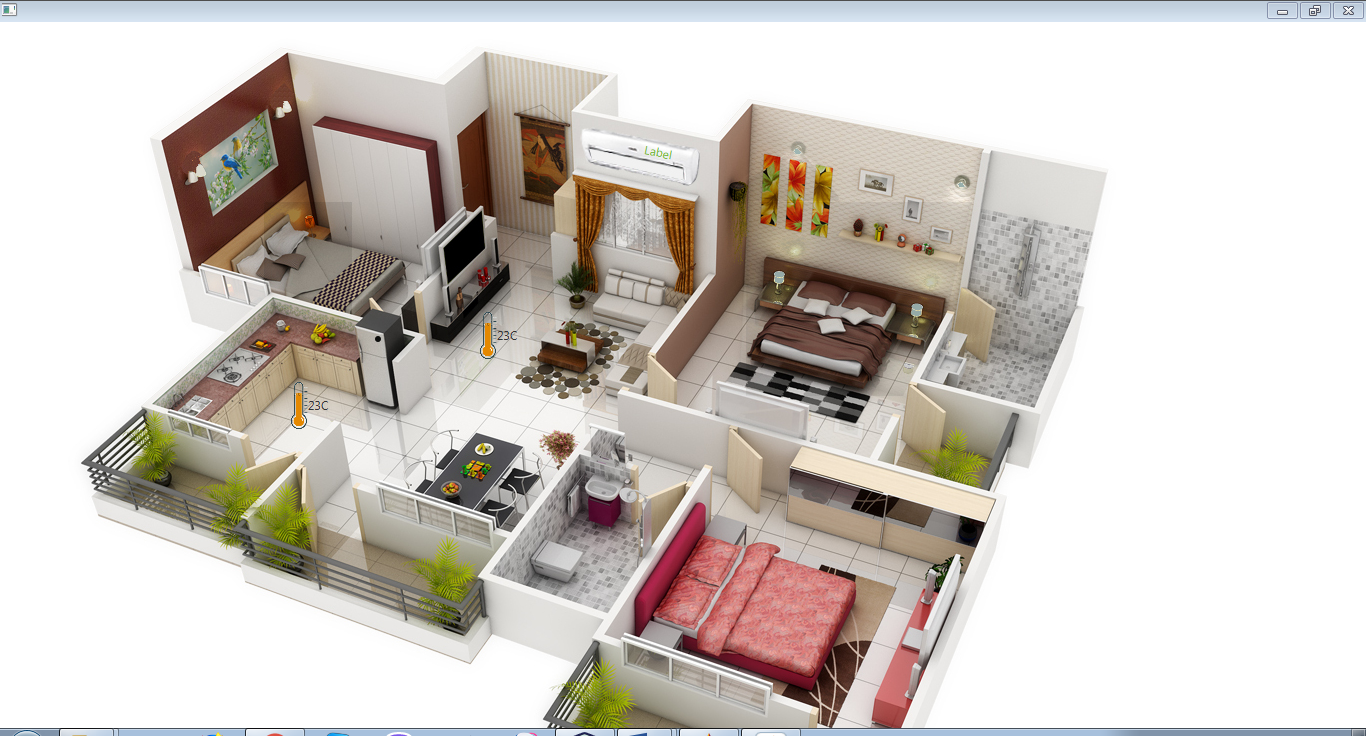
\includegraphics[scale=0.4]{chap1/fc20.png}
    \caption{LinFiSim GUI}
    \label{fc20}
\end{figure}
\subsubsection{Manipulation des états IoT VD}
Cette classe (Control) explique comment utiliser l'API du simulateur, nous appelons l'objet (L) déclaré dans le MainLinfiSim classe. Et pour changer le statut de l'IoT VD, nous appelons la méthode Set\_Name de VD\_Status (status) et passons le statut en paramètre: par exemple (voir ligne 14), nous changeons le statut de la lampe 1 en état (Status.broken). 


Pour obtenir l'etat de l'IoT VD, nous avons un appel à la méthode Get\_Name de VD\_Status (), cette méthode retourne une valeur qui définit le statut de l'IoT VD cette valeur de type "Status": par exemple (voir ligne 21).
\begin{lstlisting}
6.	import java.io.IOException;
7.	import linfisim.Status;
8.	
9.	public class Control {
10.	
11.	    public static void main(String[] args) throws IOException {
12.	
13.	           MainLinfiSim.L.Set_LAMP_1_Status(Status.broken);
14.	           MainLinfiSim.L.Set_LAMP_2_Status(Status.start);
15.	           MainLinfiSim.L.Set_TV_Status(Status.start);
16.	           MainLinfiSim.L.Set_Refrigerator_Status(Status.start);
17.	           MainLinfiSim.L.Set_AirConditioner_Status(Status.start);
18.	           MainLinfiSim.L.Set_Stove_Status(Status.start);
19.	
20.	           System.out.println(MainLinfiSim.L.Get_LAMP_1_Status());
21.	           System.out.println(MainLinfiSim.L.Get_LAMP_2_Status());
22.	           
23.	    }
24.	}

\end{lstlisting}

\begin{figure}[H]
    \centering
    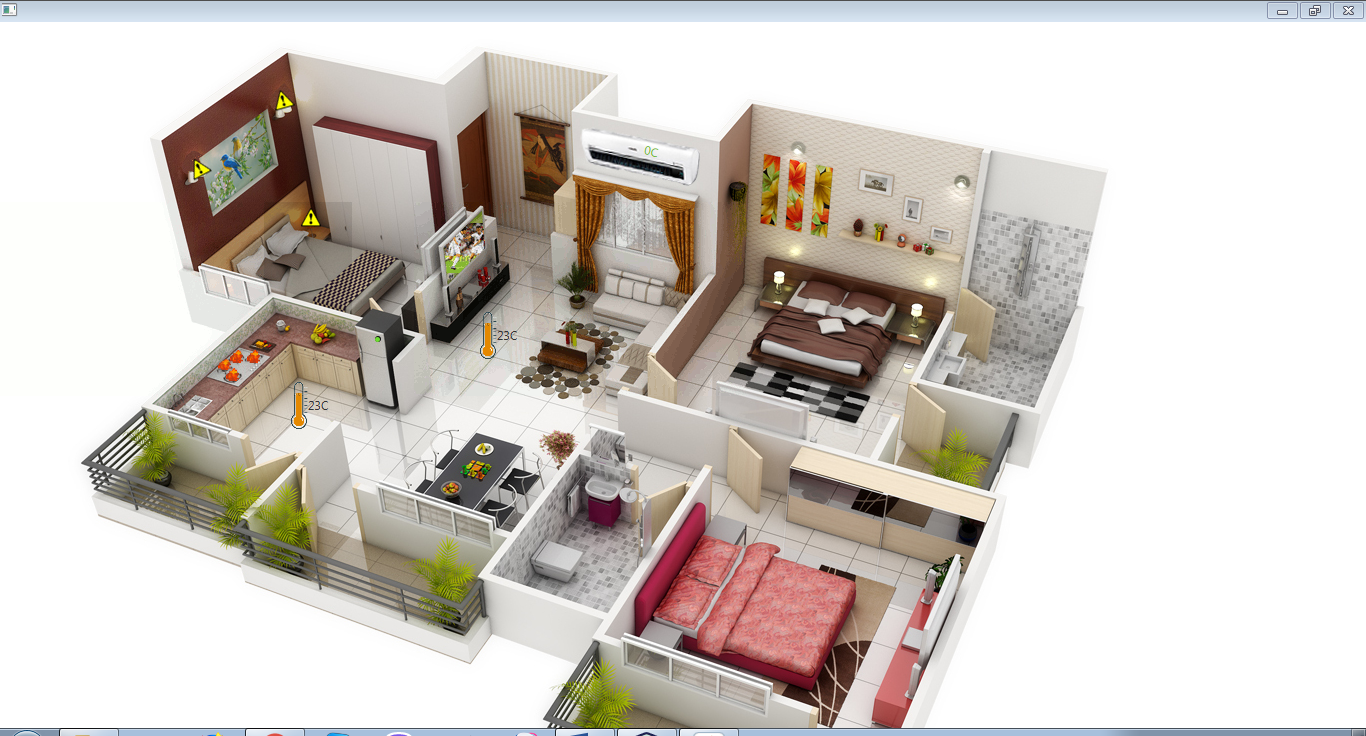
\includegraphics[scale=0.5]{chap1/fc21.png}
    \caption{IoT VD status.}
    \label{fc21}
\end{figure}

\subsubsection{Manipulation de l'IoT VS}
Ce code explique comment changer la valeur des capteurs, par exemple dans les lignes 15-16, nous définissons la valeur de la température ambiante. Et dans  la ligne 17, nous définissons la valeur de la température de la climatisation.
\begin{lstlisting}

7.	import java.io.IOException;
8.	import linfisim.Status;
9.	
10.	public class Control {
11.	
12.	    public static void main(String[] args) throws IOException {
13.	
14.	         MainLinfiSim.L.Set_AirConditioner_Status(Status.start);
15.	           MainLinfiSim.L.Set_S1_Temperature(5);
16.	           MainLinfiSim.L.Set_S2_Temperature(14);
17.	           MainLinfiSim.L.Set_AIRcondition_Temperature(14);          ;           
18.	    }
19.	}

\end{lstlisting}
\subsubsection{Afficher le tableau des statuts}
L'instruction à la ligne 14 sert à afficher la table d'état dans l'interface principale du simulateur.
\begin{lstlisting}
7.	import java.io.IOException;
8.	import linfisim.Status;
9.	
10.	public class Control {
11.	
12.	    public static void main(String[] args) throws IOException {
13.	
14.	           MainLinfiSim.L.Show_Status(true);          ;
15.	           
16.	    }
17.	}

\end{lstlisting}
\begin{figure}[H]
    \centering
    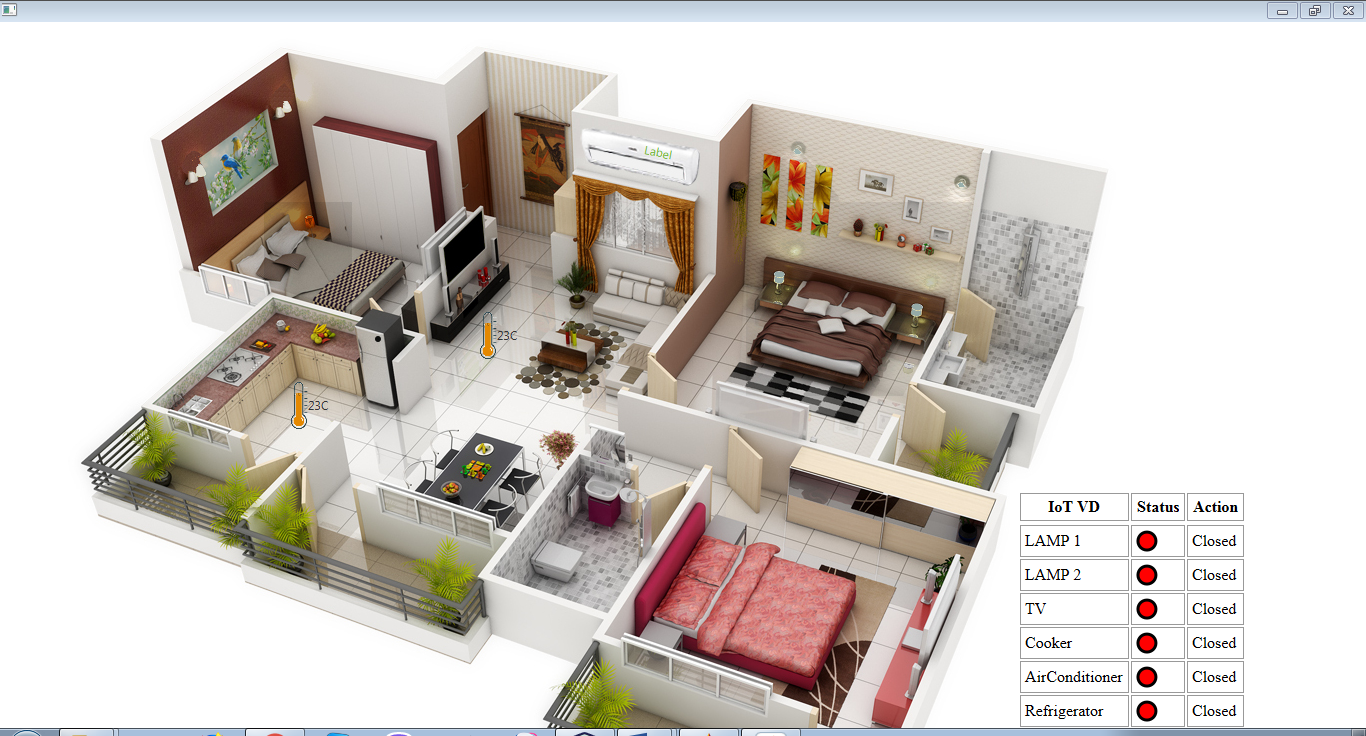
\includegraphics[scale=0.4]{chap1/fc23.png}
    \caption{API du simulateur avec la table d'état.}
    \label{fc23}
\end{figure}
\section{IoT Robot}

Dans cette section, nous présentons les pièces électroniques les plus importantes du robot. la piéce maitresse du Robot est le circuit électronique qui est lié à un moteur pour contrôler les roues du robot (avant et arrière). 

Nous avons réalisé le câblage entre les différentes unités du circuite  avec Arduino et Raspberry Pi en les attachant avec un câble série pour le transfert d'informations. 

Pour la communication Raspberry Pi et Arduino, les commandes reçues par le capteur WiFi sur le Raspberry Pi en utilisant le protocole MQTT le Raspberry Pi font une redirection des commandes vers l'Arduino via le port série (RX, TX).


\textbf{Câblage du L293D avec moteur DC: } les languettes 2, 7, 8 du L293D sont connectées aux broches 2,9 et 10 de l'Arduino, et le moteur CC avec les languettes 3,6 pour contrôler la direction du moteur (avant et arrière).


\textbf{Câblage des servomoteurs: } la broche du servo variateur est connectée à la broche Arduino 8 qui est responsable de la rotation de la caméra, ainsi que la deuxième broche du servo variateur avec la broche Arduino 7 qui est responsable de l'orientation des roues.


\textbf{Câblage complet avec l'Arduino:} Nous faisons le câblage complet avec l'Arduino, nous connectons l'anode des LED rouges avec la broche 4 et leur cathode avec (GND) et aussi l'anode des LED blanches avec la broche 3 et leur cathode avec (GND). Nous pouvons contrôler la mise sous et hors tension des LED blanches, mais les LED rouges s'allument lorsque le robot s'arrête.


 Nous avons doté le robot avec une caméra de surveillance orientable \ref{fccamera}. Il est contrôlé à distance par des commandes envoyées pas depuis smartphone. Le serveur de caméra (mouvement) envoie les images capturées à l'utilisateur en temps réel et directement. Motion est un système de surveillance assez complet. Il est extrêmement personnalisable: détection de mouvement, enregistrement image par image, enregistrement vidéo, time-laps.
\begin{figure}[H]
    \centering
    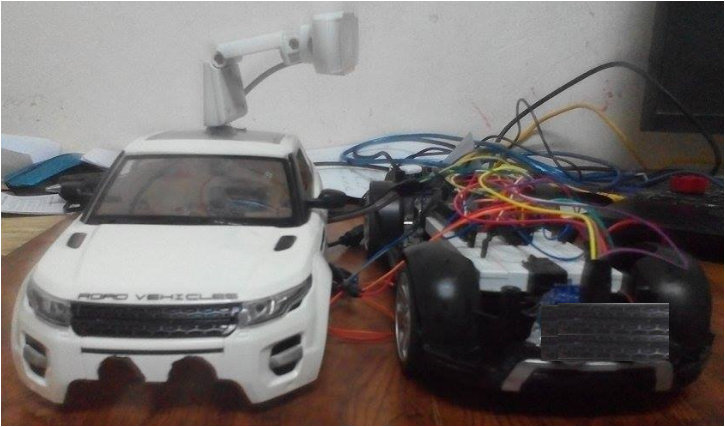
\includegraphics[scale=0.6]{chap1/fc24.png}
    \caption{Robot IoT}
    \label{fccamera}
\end{figure}

\section{IoT device}
Nous avons implémenté notre architecture pour créer un dispositif IoT de sécurité. Ceci, enfin, contrôle la sécurité d'un environnement contre les événements accidentels. Son objectif est d'agir sur l'existence d'un criminel dans l'environnement. Et il peut contrôler les risques d'accidents tels que les incendies et les fuites de gaz. La mise en œuvre est illustrée à la figure \ref{fc16} et expliquée ci-dessous.


Nous implémentons notre architecture proposée avec les cartes Raspberry pi 2 (voir le côté gauche sur la figure \ref{fc16}), où cette carte nous a permis de combiner les trois couches suivantes en une seule structure (comme indiqué sur le côté droit de la figure \ref{fc16}):
\begin{itemize}
    \item \textbf{la couche application:} il s'agit d'une application d'un véritable environnement de sécurité (maison, appartement, beurre, lieu de travail);
\item \textbf{	La couche d'agent:} c'est un agent embarqué (voir figure \ref{fc9}) dans le dispositif IoT, il gère les informations reçues par les capteurs, analyse ces informations et prend des décisions;
\item \textbf{Couche de communication réseau et données:} le périphérique IoT communique avec les autres périphériques via cette couche;
\item \textbf{Sensing Layer :} il a été implémenté sur le capteur de présence et l'humidité et capteur de température. La figure \ref{fc9} montre l'architecture particulière de l'agent de sécurité;
\item \textbf{Environnement:} il est constitué par l'environnement réel (maison, appartement, lieu de travail), il contient les composants d'un utilisateur et voisins (l'autre composant situé au même endroit).
\item \textbf{capteurs:} il s'agit d'un appareil qui permet de transformer l'état d'une grandeur physique observée (environnement) en une grandeur utilisable (mesures). Tels qu'une tension électrique, une hauteur de mercure, une intensité ou la déviation d'une aiguille. Il y a souvent une confusion entre le capteur et le transducteur: un capteur est au moins composé d'un transducteur;
\item \textbf{Base historique des États:} c'est un outil pour stocker l'historique des informations fournies par les capteurs (l'état de l'environnement) et les états des autres composants du système;
\item \textbf{Base de règles:} il rassemble les connaissances de l'agent. Il contient des règles pour aider l'agent à prendre des décisions. De telles décisions modifient son statut sur l'état actuel de l'environnement et les statuts d'autres agents. La base de règles est mise à jour en fonction des nouveaux états et besoins de l'environnement. Les règles qui représentent les connaissances générales sur la sécurité et les conclusions factuelles.

\end{itemize}



Nous avons implémenté notre architecture en utilisant Raspberry PI Model B et le système d'exploitation Raspbian. Avec eux, nous avons créé l'appareil IoT qui lance l'agent de sécurité intégré à l'appareil pour assurer la sécurité de l'environnement contre les événements accidentels et fortuits associés à un module sans fil pour la communication de l'appareil avec les autres appareils et avec Internet.


Nous avons implémenté notre agent de sécurité via le JADE (Java Agent Development Framework). Il simplifie la mise en œuvre de systèmes multi-agents grâce à un middleware conforme aux spécifications de la Foundation for Intelligent Physical Agents (FIPA)  et à travers un ensemble d'outils graphiques qui prennent en charge les phases de débogage et de déploiement.


Nous utilisons deux types de capteurs pour fournir la couche de détection: un capteur de mouvement PIR (HCSR501 PIR) pour détecter la présence d'une personne (intrus) dans l'environnement et un capteur de gaz pour détecter les fuites de gaz à l'emplacement. Nous avons connecté des capteurs électroniques au Raspberry Pi Model B. De plus, nous les avons contrôlés avec Java en utilisant une entrée / sortie à usage général (GPIO).

\subsection{Composantes électroniques de IoT device}
Cette section représent l'ensemble des pièces électroniques  responsables de la transformation (capteurs), de l'analyse, du traitement (Raspberry PI) et du transfert (module de communication) de l'état d'une grandeur physique observée en quantité utilisable.
\subsubsection{PIR Motion Sensor (HCSR501 PIR)}
PIR sensors (Figure \ref{ceiotdev}) nous permettent de détecter le mouvement  et ils sont toujours utilisés pour détecter si un humain est entré / sorti de la plage des capteurs. Ils sont petits, peu coûteux, de faible puissance, faciles à utiliser et ne s'usent pas. Pour cette raison, ils se trouvent généralement dans les appareils et gadgets utilisés dans les maisons ou les entreprises. Ils sont souvent appelés capteurs PIR, «infrarouge passif», «pyroélectrique» ou «mouvement PIR».
\subsubsection{Capteur d'humidité et de température (DHT-11)}
Figure \ref{ceiotdev} montre le module de capteur d'humidité et de température et est basé sur le capteur DHT-11 , qui est un capteur de température et d'humidité numérique très populaire et à très bas prix. Il utilise un capteur d'humidité capacitif et une thermistance pour mesurer la température de l'air ambiant. Le résultat est disponible via un signal numérique sur la broche de données (aucune broche d'entrée analogique n'est nécessaire). Il peut mesurer l'humidité de 20 à 80\% des lectures d'humidité avec une précision de 5\% et des lectures de température de 0 à 50 ° C avec une précision de ± 2 ° C.

\subsubsection{Raspberry Pi Model B}
Figure \ref{ceiotdev} montre le Raspberry Pi Model B  qui est une petite version d'un ordinateur exécutant le système d'exploitation Linux sur carte SD pour une application informatique intégrée. En raison de ses caractéristiques, la couche d'agent de déploiement dans l'appareil et le fonctionnement sont la capacité de stockage et de traitement pour améliorer les performances dans lesquelles cette carte est équipée :
\begin{itemize}
    \item	Broadcom BCM2836 processor, four 900 MHz ARMv7 cores;
\item 1 GB of DDR2 memory;
\item Ethernet / RJ45 port, 10.100 BaseT is connect Raspberry Pi to a network;
\item Four USB 2.0 ports;
\item HDMI video output for connecting a display;
\item Taken for camera;
\item 40 pins GPIO connectors (all running at 3.3 V);
\item Memory card port: 1 micro SD port is used as a storage medium;
\item 1 Micro USB for power supply;
\item Analogue audio connectors: 1 3.5mm jack output;
\end{itemize}

\subsection{Câblage et circuit éléctronique}
Après avoir  preparé les composants électroniques et la carte Raspberry PI , nous devons connecter les pièces nécessaires pour rendre le système opérationnel (voir figure \ref{ceiotdev}). 


\begin{figure}[H]
    \centering
    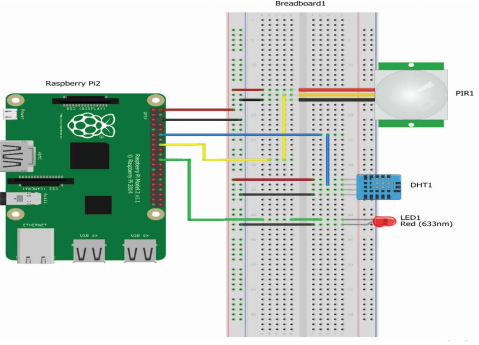
\includegraphics[scale=1.2]{chap1/fc26.png}
    \caption{Circuit éléctronique de IoT device}
    \label{ceiotdev}
\end{figure}
\subsection{Fonctionnalités  de IoT device }
Pour tester notre application , nous avons collecté les informations (température l'humidité) dans la période 19-20 décembre 2017 dans la ville de Biskra, Algérie.

Le système travaille de maniére continue est independante,  détecte la température et l'humidité de l'environnement, puis stocke les données dans sa propre base de données. Il avertit également l'utilisateur en cas de changements importants de température et d'humidité. 

En plus il protège également l'environnement contre les intrus en l'absence de l'utilisateur lorsque le système avertit l'utilisateur.

La figure \ref{fc27} montre la température et l'humidité détectées par le systeme ainsi que la detection d'un intrus dans le smart house.
\begin{figure}[H]
    \centering
    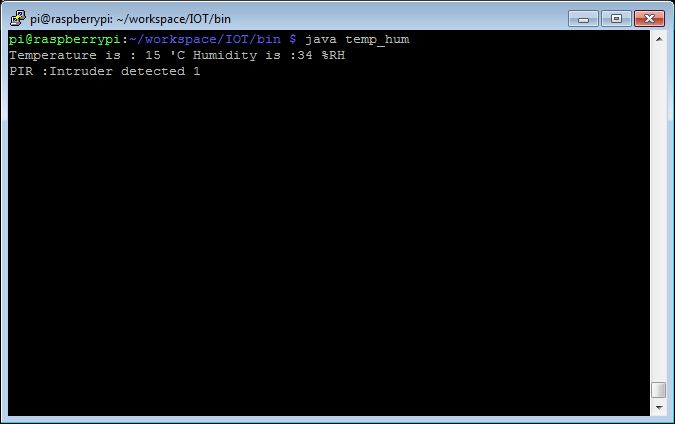
\includegraphics[scale=0.8]{chap1/fc27.png}
    \caption{Agent sécurité IoT détecte la présence d'une personne à la maison.}
    \label{fc27}
\end{figure}

La courbe suivante résume les changements de température et d'humidité dans l'atmosphère capturés en 24 heures, la température est comprise entre 6 et 15 degrés tandis que l'humidité est comprise entre 35 et 68 degrés.

\\
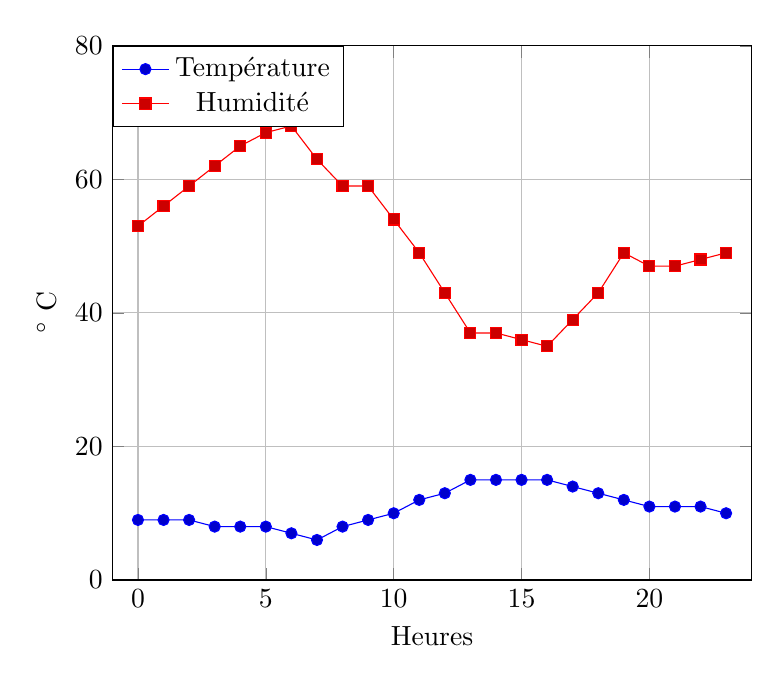
\begin{tikzpicture}
		\begin{axis}[	grid= major ,
				width=0.8\textwidth ,
				xlabel = {Heures} ,
				ylabel = {$^\circ$ C} ,
				xmin = -1, xmax = 24,
				ymin = 0, ymax = 80,
				legend entries={Température, Humidité},
				legend style={at={(0,1)},anchor=north west}]
			\addplot coordinates {(0,9) (1,9) (2,9) (3,8) (4,8)(5,8)(6,7) (7,6)(8,8)(9,9) (10,10) (11,12)(12,13)(13,15)(14,15) (15,15)(16,15)(17,14) (18,13) (19,12)(20,11)(21,11) (22,11)(23,10) }; % Tracé point à point
		\addplot coordinates {(0,53) (1,56) (2,59) (3,62) (4,65)(5,67)(6,68) (7,63)(8,59)(9,59) (10,54) (11,49)(12,43) (13,37)(14,37) (15,36)(16,35)(17,39) (18,43) (19,49)(20,47)(21,47) (22,48)(23,49) };
		%\caption{Courbe de température et d'humidité capturée pendant 24 heures.}
		\end{axis}
			\end{tikzpicture}

		La fenêtre suivante explique l'échange de messages entre les agents, l'agent "IoT security" n'envoie pas de message aux autres agents car il ne détecte aucun danger dans l'environnement.
		\begin{figure}[H]
    \centering
    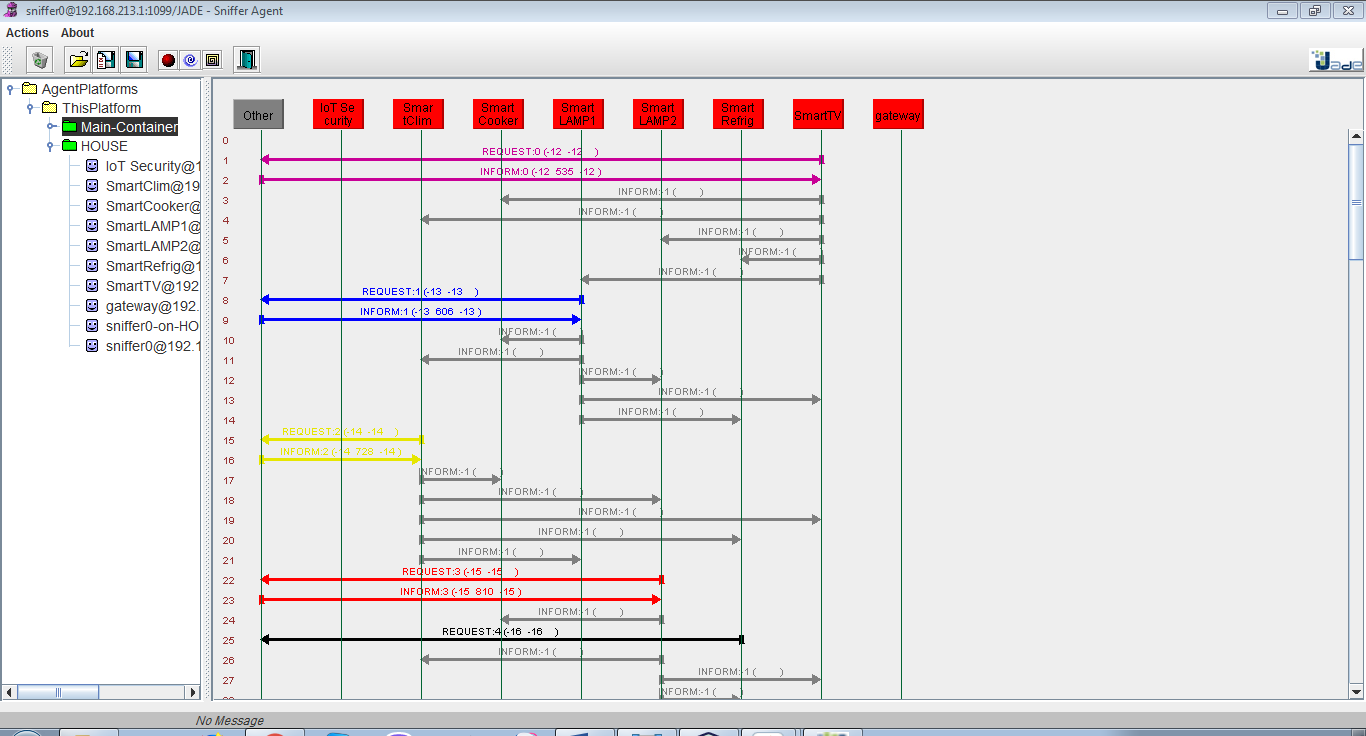
\includegraphics[scale=0.4]{chap1/fc28.png}
    \caption{Communication entre agents}
    \label{fc28}
\end{figure}


La fenêtre suivante explique la réaction de l'agent "sécurité IoT" après la détection d'une personne dans l'environnement et le mode de surveillance est à l'état actif.


L'agent «sécurité IoT» a diffusé un message de «demande de réaction» et chaque agent reçoit ce message qui répondra par l'action appropriée à la demande.
	\begin{figure}[H]
    \centering
    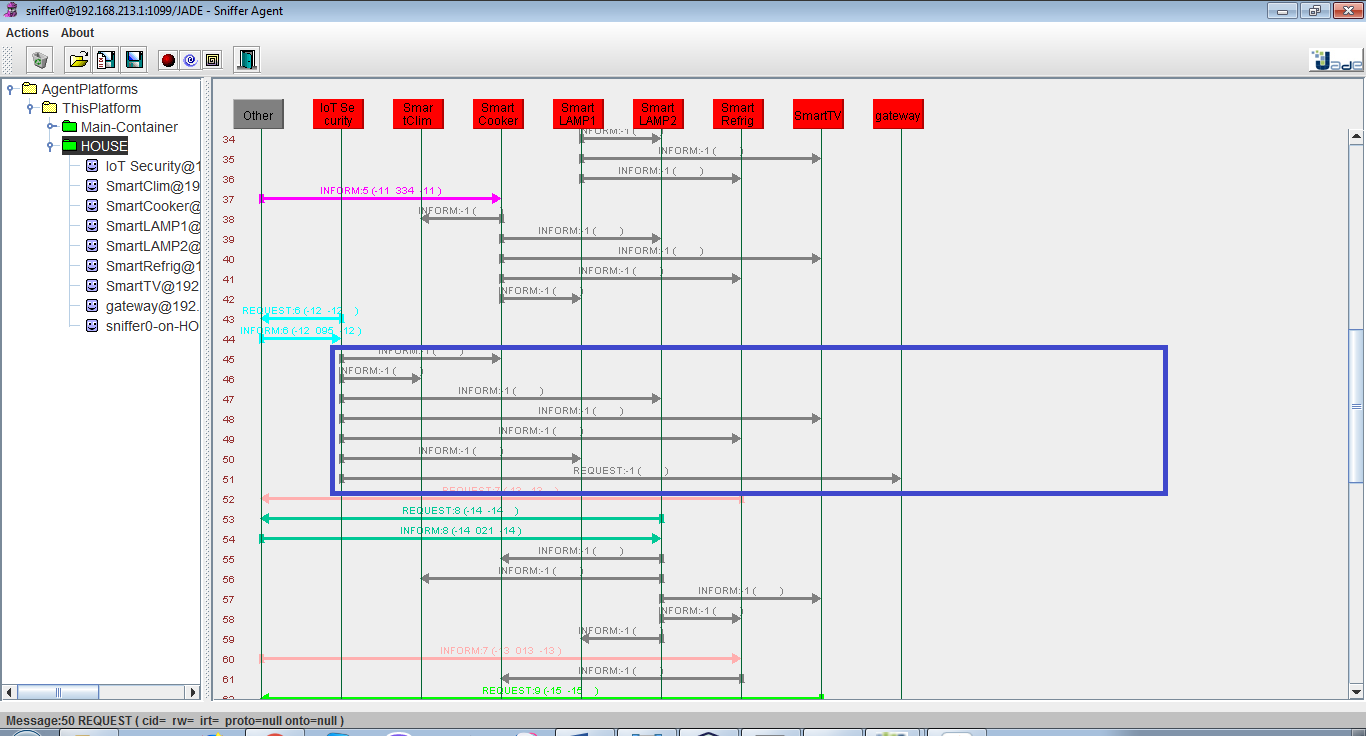
\includegraphics[scale=0.5]{chap1/fc29.png}
    \caption{Réaction de l'agent sécurité IoT}
    \label{fc29}
\end{figure}

L'agent alerte également l'utilisateur avec un message envoyé au smartphone. La figure suivante montre le message que l'utilisateur reçoit immédiatement après que l'appareil détecte un intrus dans la maison.
		\begin{figure}[H]
    \centering
    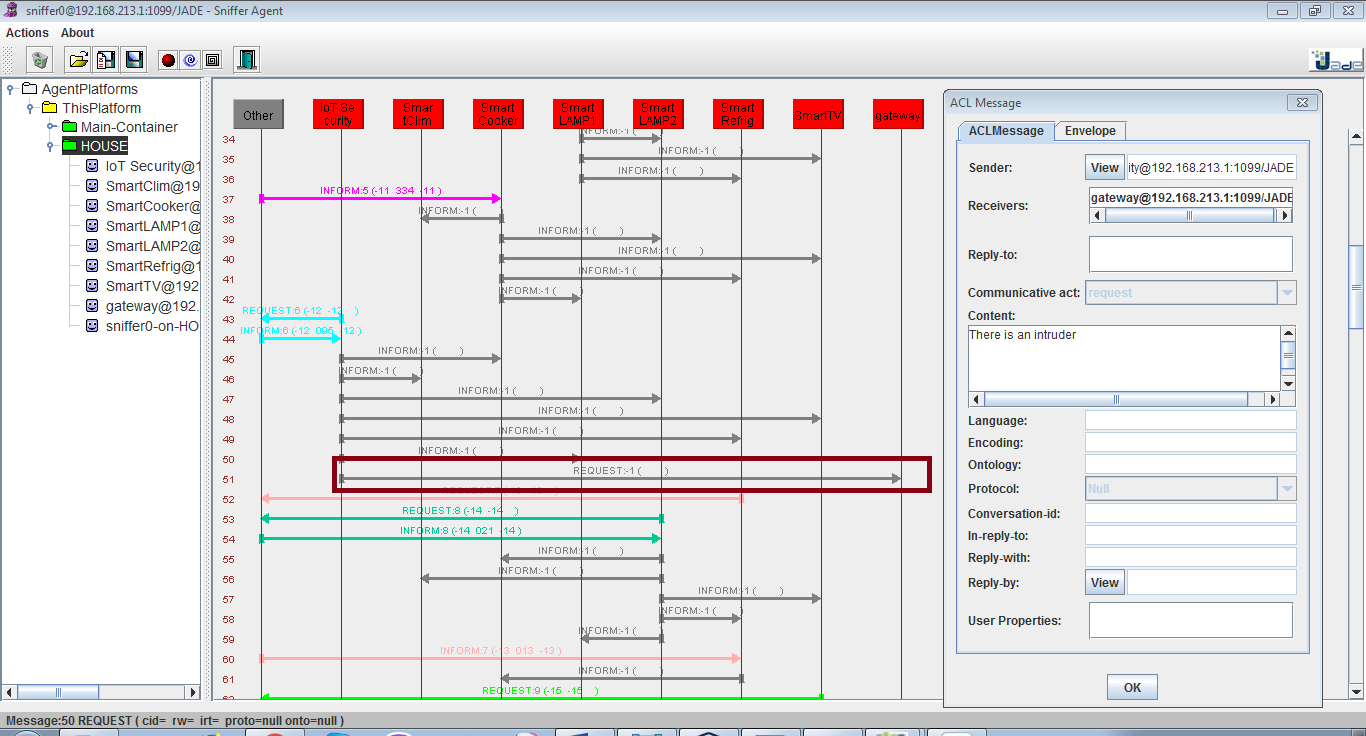
\includegraphics[scale=0.5]{chap1/fc30.png}
    \caption{Agent de sécurité IoT envoie un message à l'utilisateur.}
    \label{fc30}
\end{figure}
%\section{Résultats}
\section{Conclusion}

Ce chapitre a été consacré à l'implémentation de notre solution IoT. Au début nous avons présenté les outils et platformes utilisés.

Nous avons commencé par l'implémentation su simulateur smart house où nous avons expliqué et clarifié certaines méthodes. Nous avons montré comment utiliser l'API de simulateur et comment manipuler les capteurs IoT.

Dans la seconde implémentation , nous avons présenté l'IoT Robot ,ses composants éléctroniques et son fonctionnement.

Enfin, nous avons terminé ce chapitre par l'implémentation de l'IoT device dont nous avons présenté les composants éléctronique et aussi le fonctionnement logicel de l'IoT device.


